\documentclass[sigconf]{acmart/acmart}
\usepackage{lipsum}

\AtBeginDocument{%
    \providecommand\BibTeX{{%
                Bib\TeX}}}

\begin{document}
\title{Recent Progress}
\author{sailing-innocent}
\authornote{updated March 19th. 2023}
\email{some@email}

\affiliation{%
    \institution{Jialidun University}
    \streetaddress{Some Where on Earth}
    \city{The City}
    \state{The State}
    \country{The Country}
    \postcode{xxxxxx}
}
\begin{abstract}
    \lipsum[3]
\end{abstract}

\keywords{AIGC, Geometric Deep Learning, Terrain Generation, 3D Reconstruction, Multi-view Synthesis}
%% A "teaser" image appears between the author and affiliation
%% information and the body of the document, and typically spans the
%% page.
\begin{teaserfigure}
    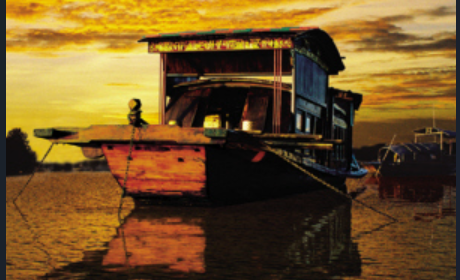
\includegraphics[width=\textwidth]{fig_boat.png}
    \caption{Boat}
    \Description{The Boat}
    \label{fig:teaser}
\end{teaserfigure}

\maketitle

\paragraph{Machine Learning:}

\lipsum[10]

%%
%% The next two lines define the bibliography style to be used, and
%% the bibliography file.
\bibliographystyle{acmart/ACM-Reference-Format}

\end{document}
\endinput
